\begin{figure*}
\centering
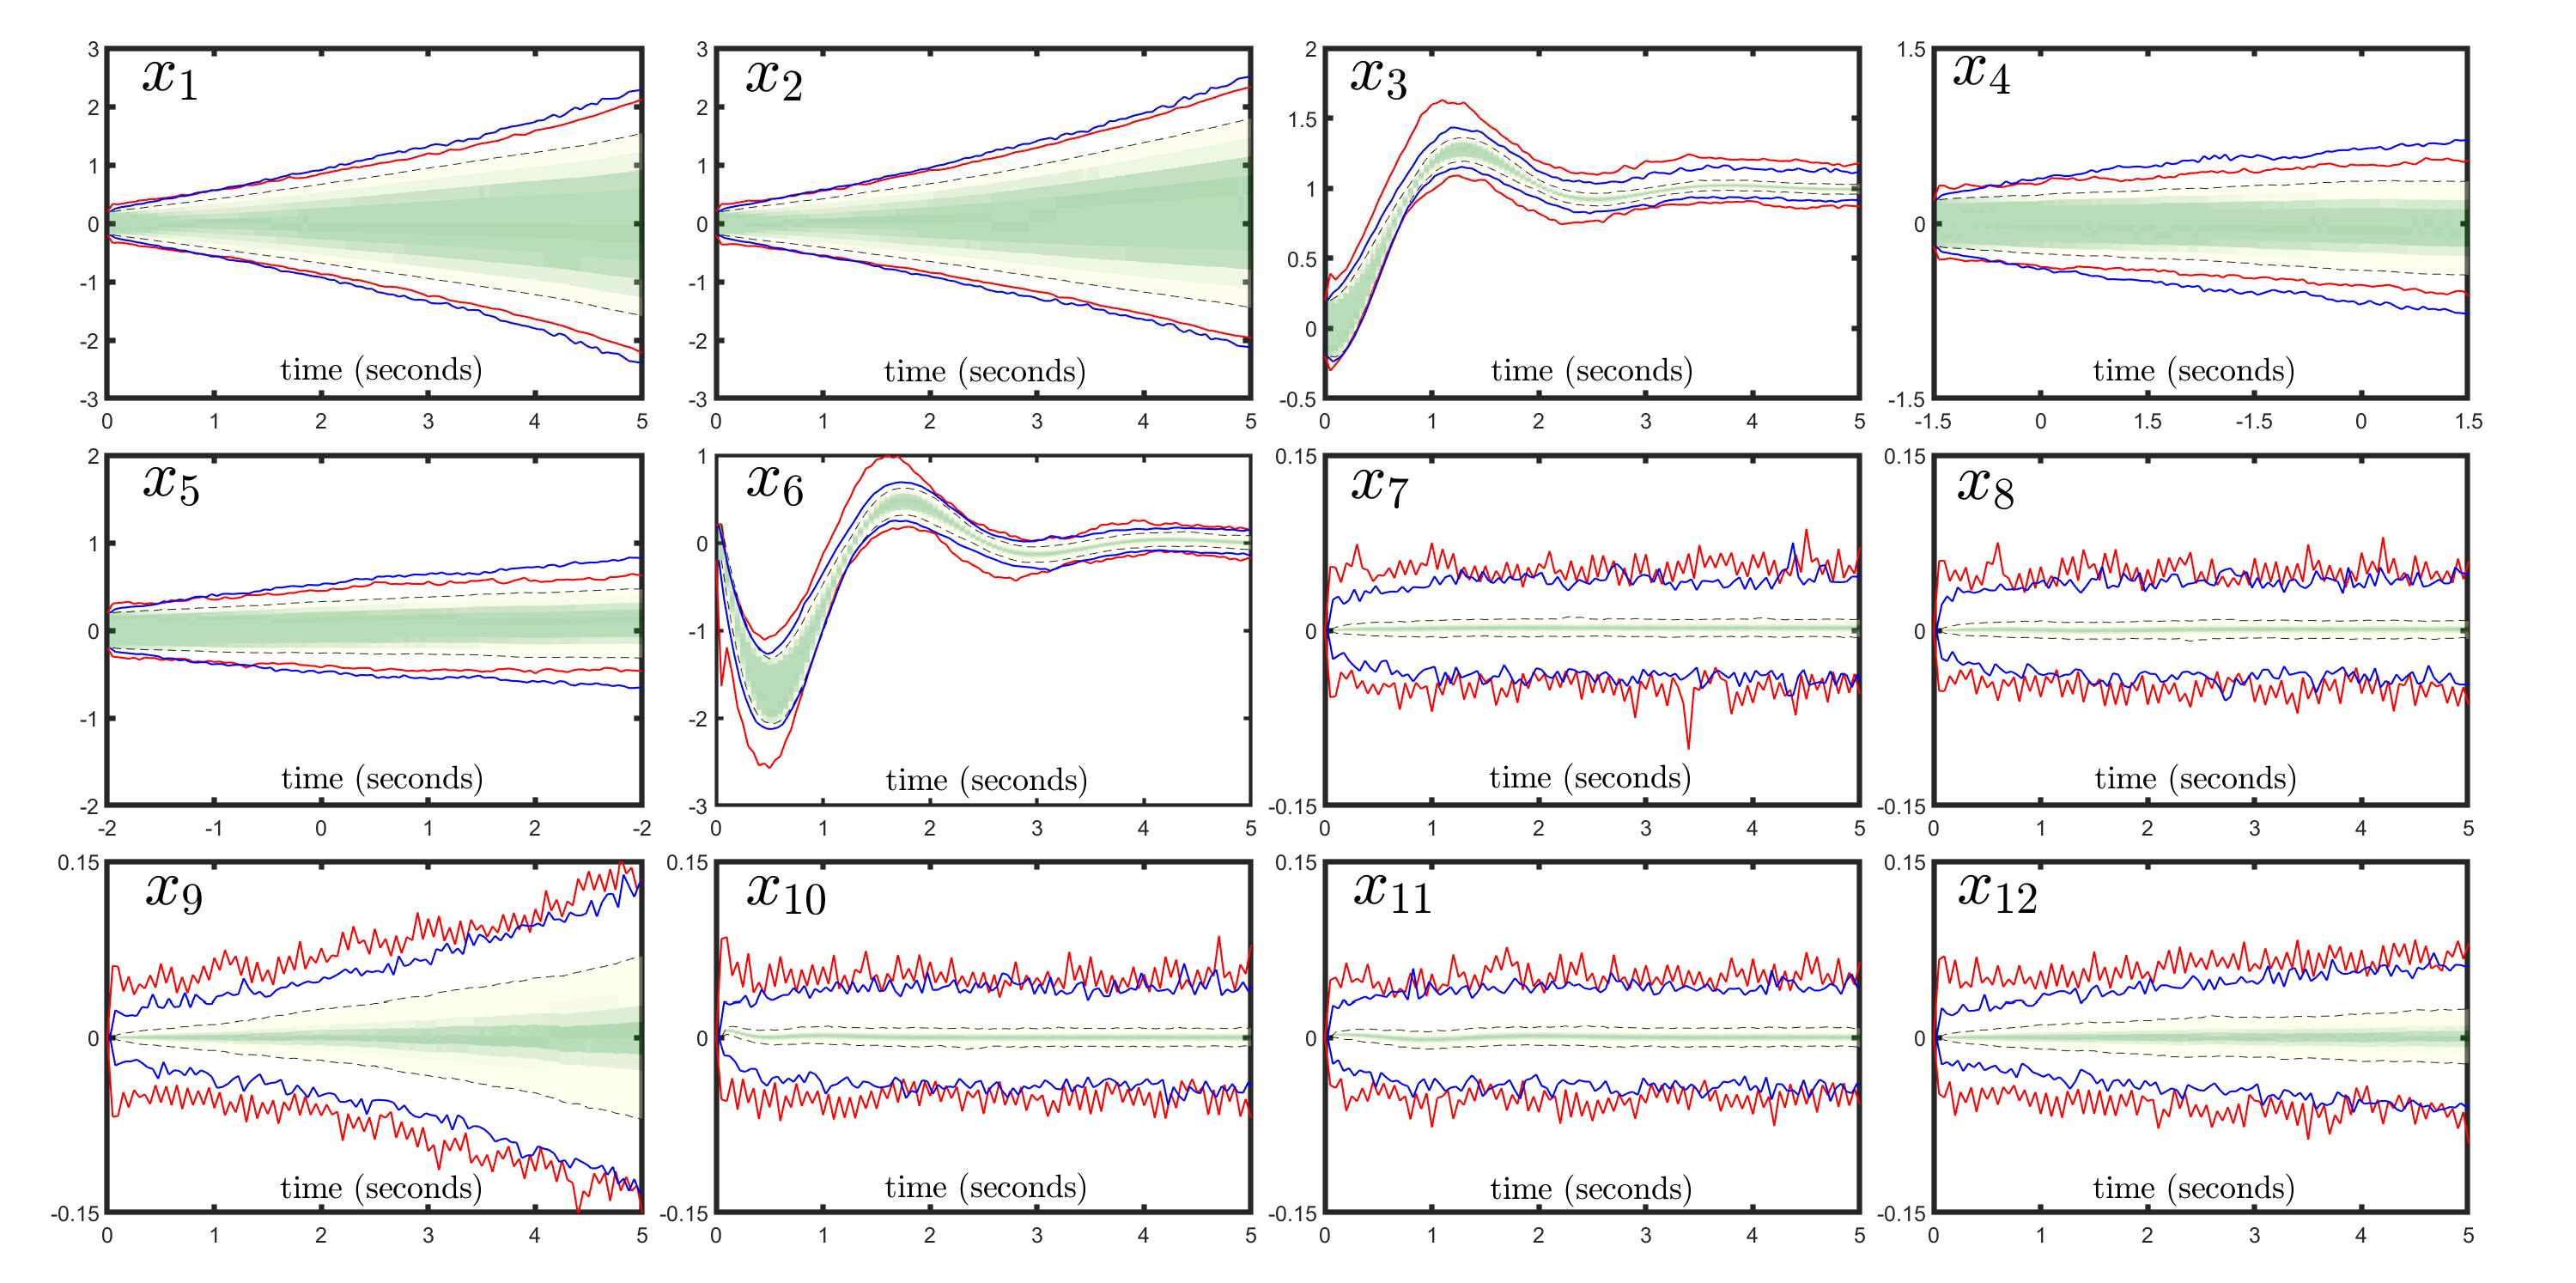
\includegraphics[trim={3.6cm
  1cm 3.7cm 1cm},width =0.85\linewidth]{figures/AAAI_comaprison.pdf}
% \includegraphics[width =0.85\linewidth]{figures/compare_with_EMSOFT_True.pdf}
\caption{Shows the comparison with \cite{hashemi2024statistical}. The blue and red borders are projections of our and their $\delta$-confident flowpipes respectively with $\delta = 99.99\%$. The shaded regions show the density of the trajectories from $\traindataset$.}
\label{fig:compEmsoft}
\end{figure*}
\begin{figure*}
\centering
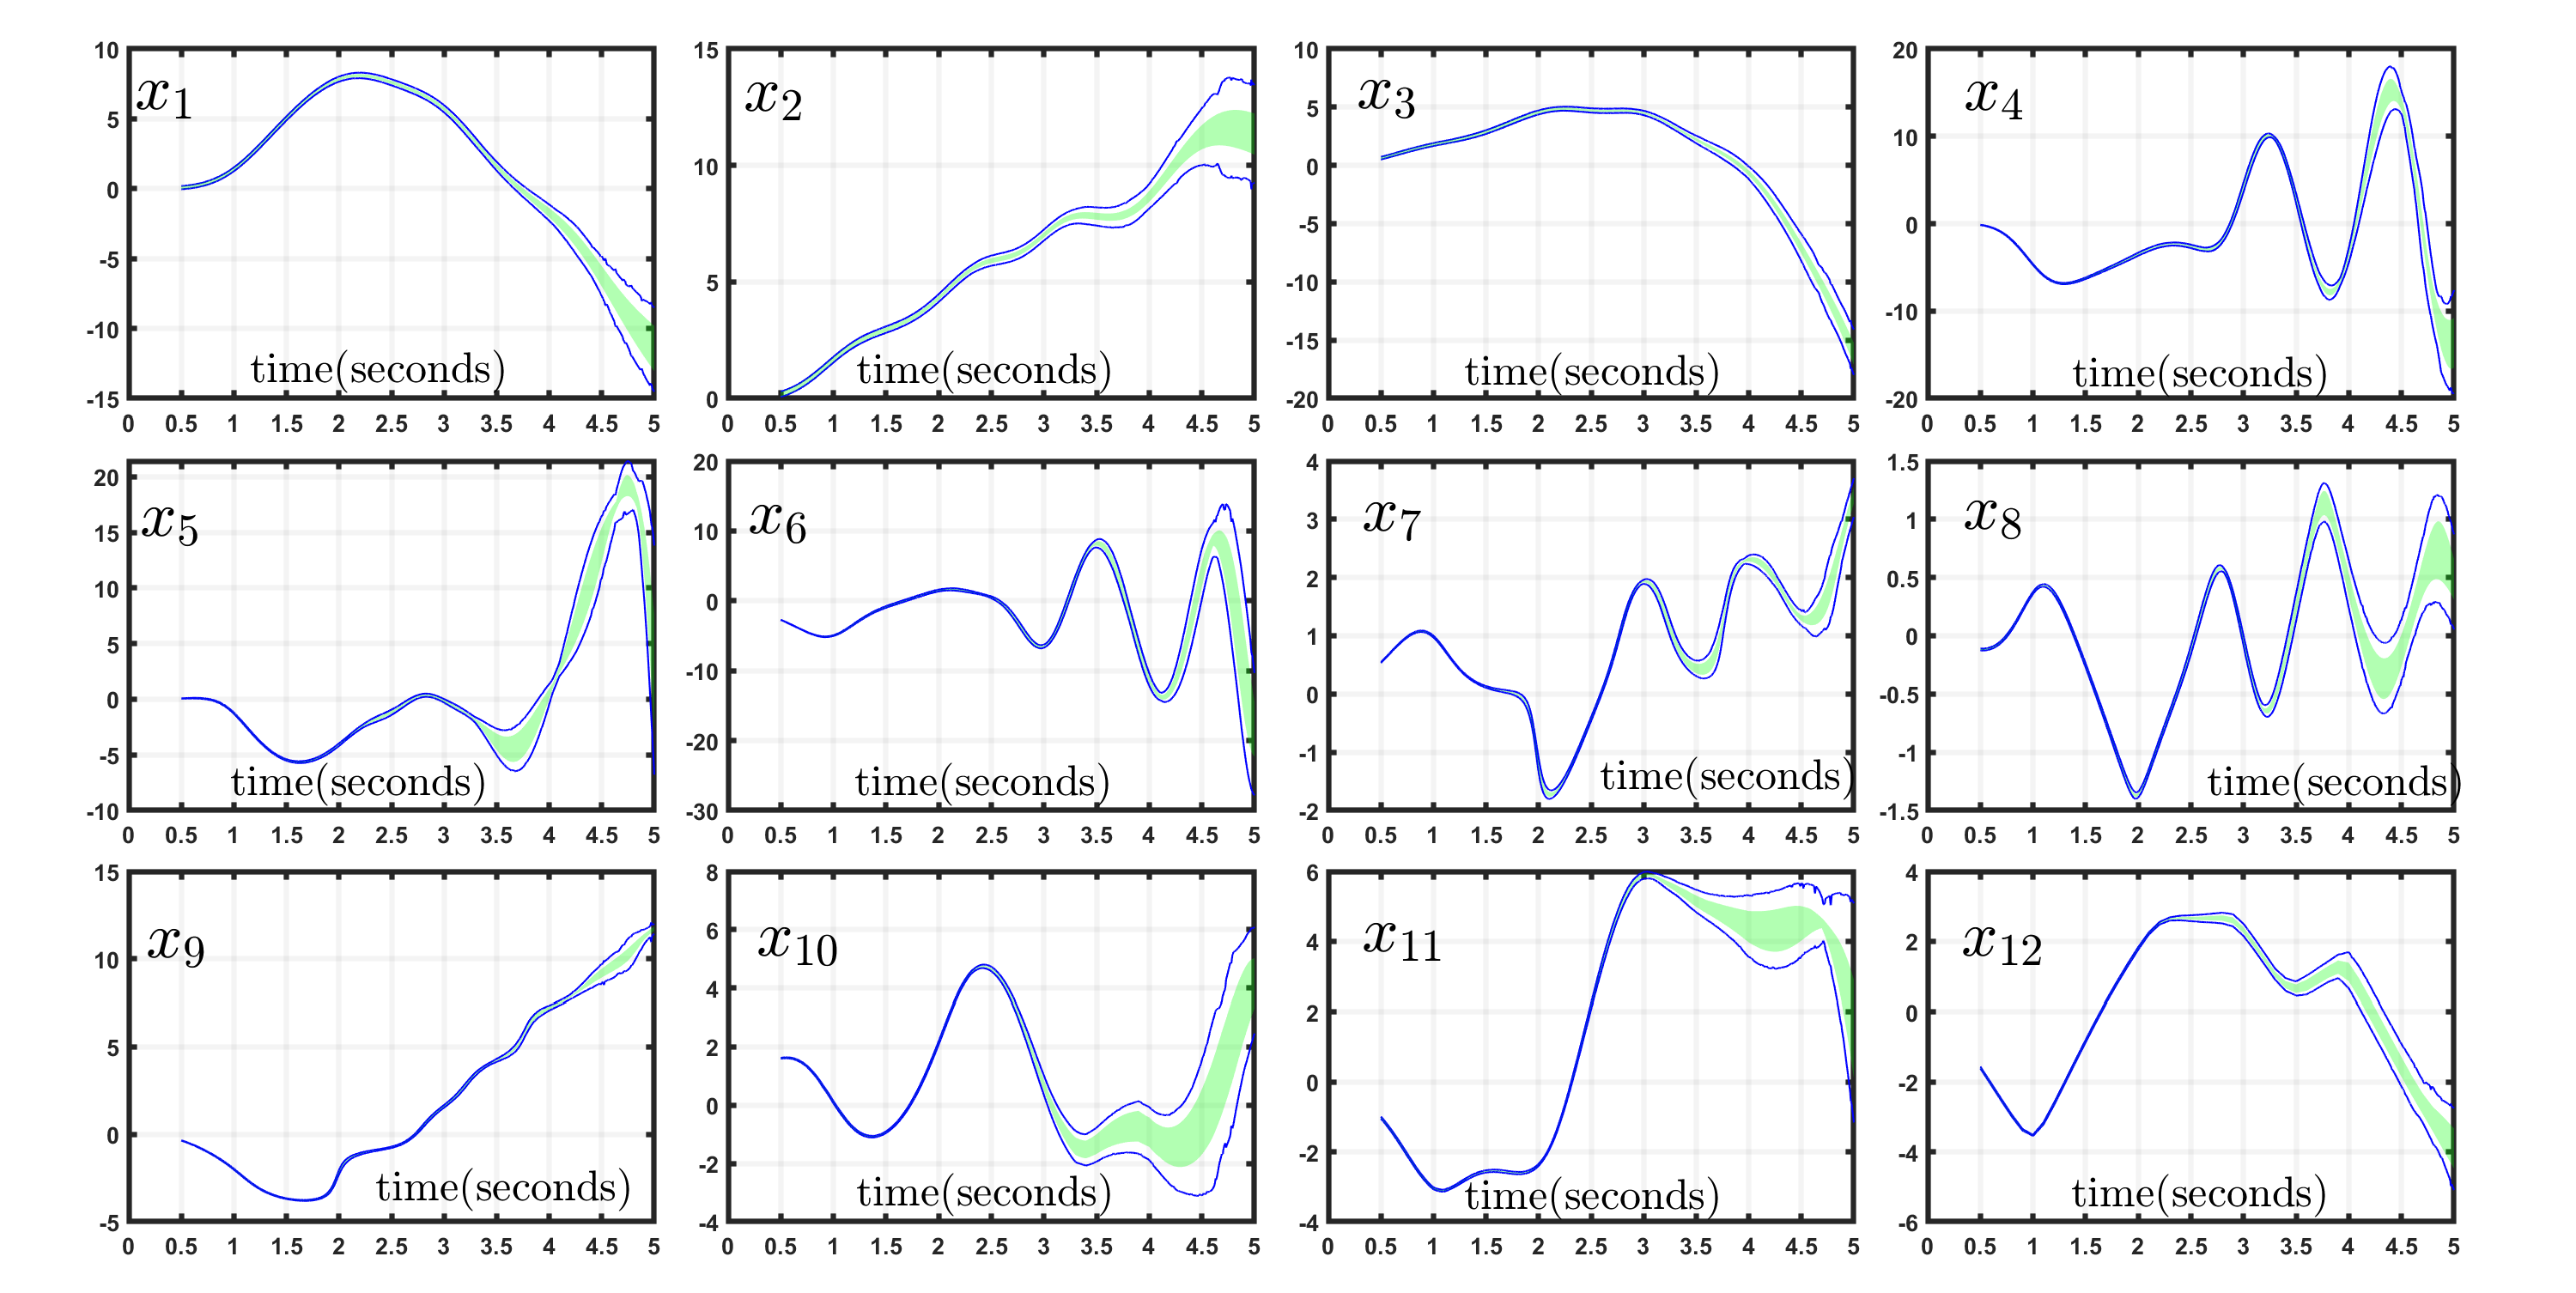
\includegraphics[trim={3.6cm
  1cm 3.4cm 1cm},width =0.85\linewidth]{figures/results_True_pretty.pdf}
% 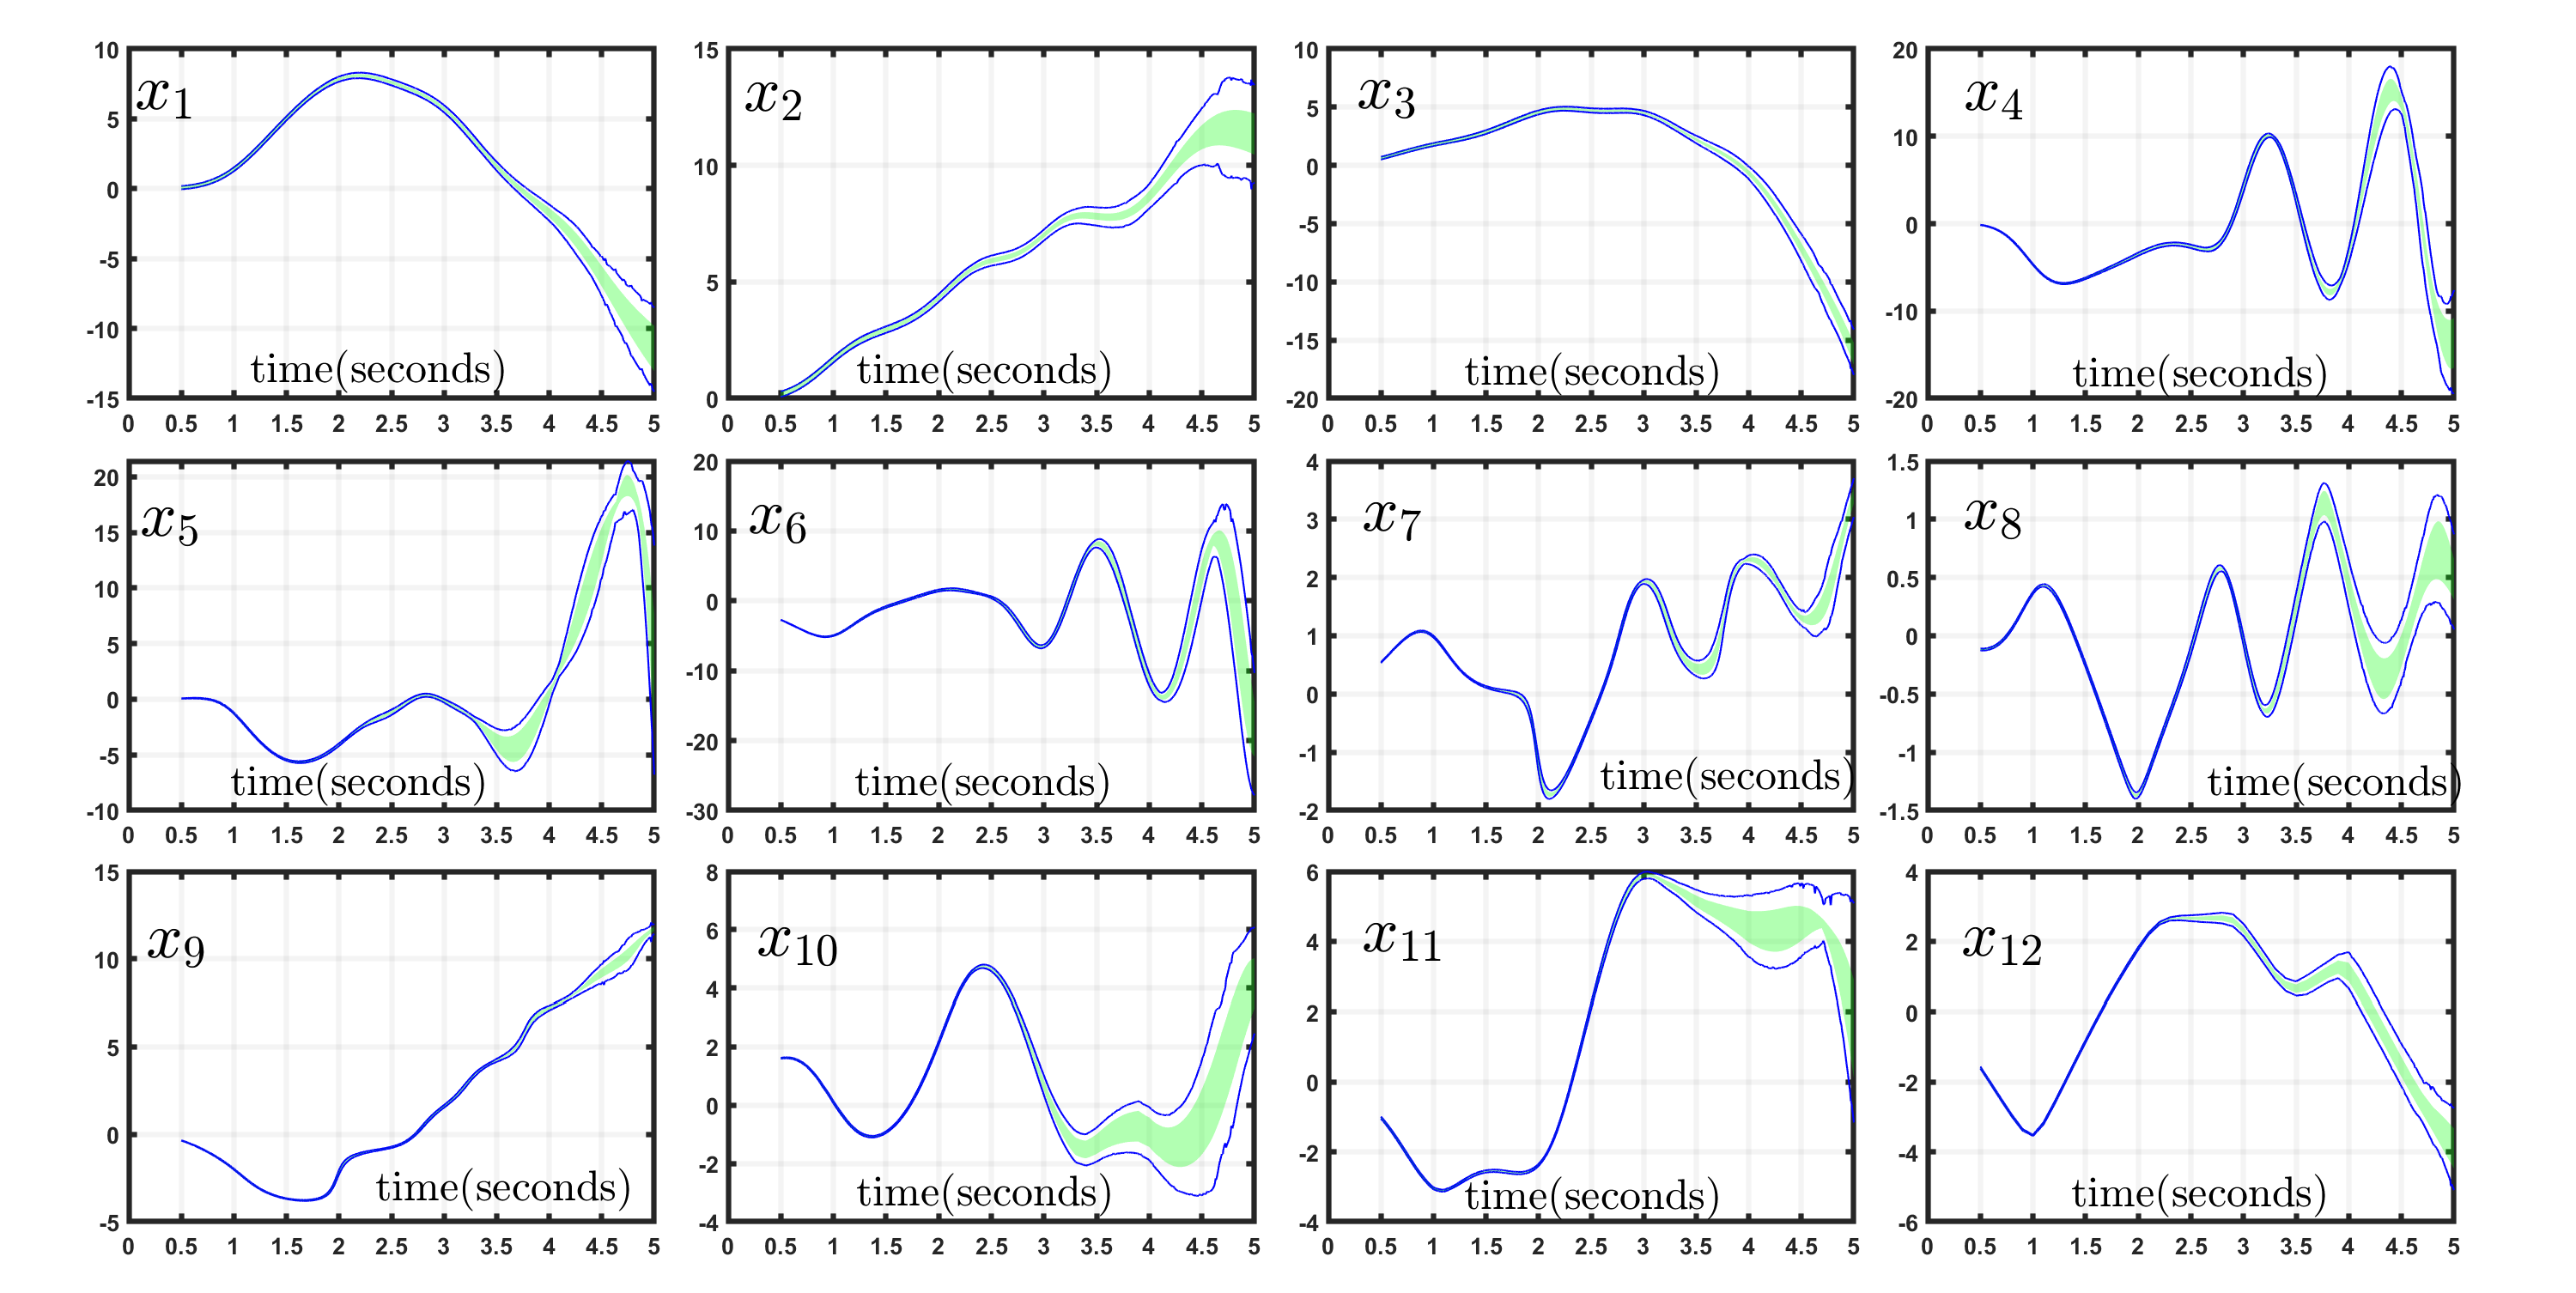
\includegraphics[width =0.85\linewidth]{figures/results_True_pretty.pdf}
\caption{ Shows the projection of our $\delta$-confident flowpipe on each component of the trajectory state. The shaded area are the simulation of trajectories from $\traindataset$.}
\label{fig:nested}
\vspace{-5mm}
\end{figure*}

\begin{figure*}
    \begin{minipage}[t]{0.76\textwidth}
        \centering
        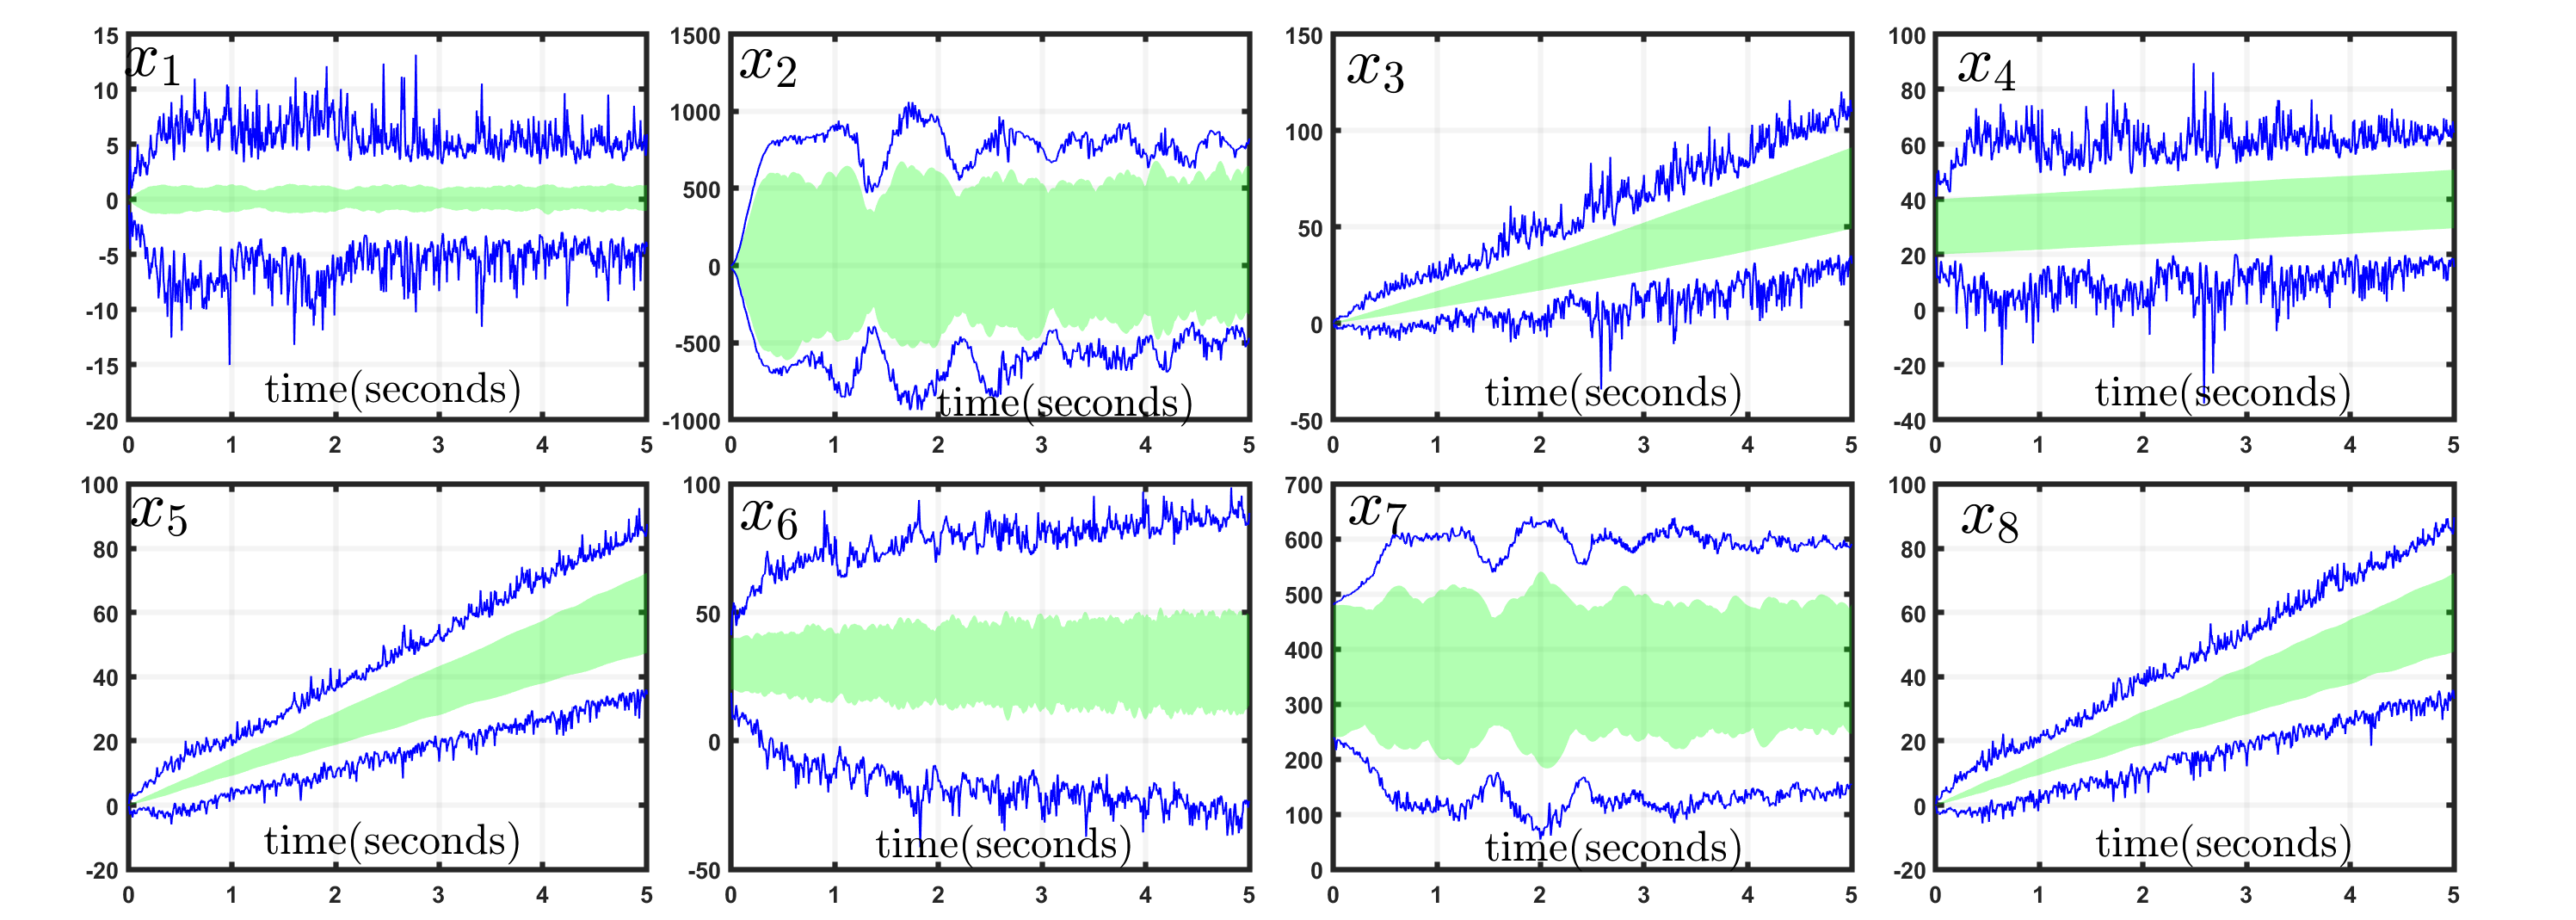
\includegraphics[trim={3.2cm 0.5cm 3.4cm 2cm},width = 0.95\textwidth]{figures/First_8_states2.pdf}
        \caption{Shows the projection of our $\delta$-confident flowpipe on the first $8$ components of the trajectory state. There is a shift between the distribution of deployment and training environments. The shaded area are the trajectories sampled from the deployment environment.}\label{fig:proj}
    \end{minipage}
    \hfill
    \begin{minipage}[t]{0.21\textwidth}
        \vspace{-4.5cm}
        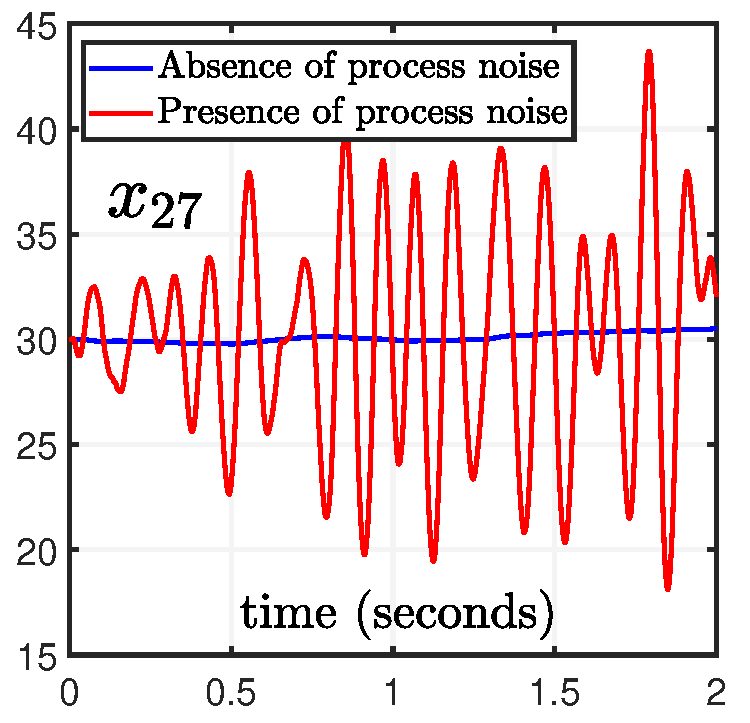
\includegraphics[width=\textwidth]{figures/noise_contribution.pdf}
        \caption{Shows the comparison of angular velocity of the last rotating mass in presence and absence of the process noise.}
        \label{fig:noisecontribution}
    \end{minipage}
    \vspace{-5mm}
\end{figure*}
\section{Detail of the Experiments}
\subsection{Experiment 1:[Comparison with \cite{hashemi2024statistical}]} Here we address Experiment 2 from \cite{hashemi2024statistical} for comparison of the results. In this experiment, a quadcopter hovers at a specific elevation, and its trajectories are simulated over a horizon of $\horizon = 100$ time steps, with a sampling time of $\delta t = 0.05$. The $\delta$-confident flowpipe has a confidence level of $\delta = 99.99\%$. Compared to \cite{hashemi2024statistical}, our approach achieves a higher level of accuracy. This improvement is due to our training strategy, which allows us to use exact-star for surrogate reachability, and our PCA-based technique, which results in smaller inflating hypercubes. In this experiment, we use a trajectory division setting of $N=100$, $T_q=1$, for $q\in[N]$, with $\relu$ neural network surrogate models structured as $[12, 24, 12]$. Figure \ref{fig:compEmsoft} shows the projection of the flowpipe on each state in comparison with the results of \cite{hashemi2024statistical}, and Table \ref{tbl:expdetails} shows the detail of the experiment.

\subsection{Experiment 2: [Sequential Goal Reaching Task]} In this example, we consider the quadcopter scenario described in \cite{hashemi2024scaling}, where a controller is designed to ensure that the machine accomplishes a sequential goal-reaching task. We also include the previously mentioned process noise in the simulator to include stochasticity. Given the quadcopter's tendency for unpredictable behavior, we significantly reduce the sampling time in this instance. The trajectories are sampled at a frequency of 1 KHz over a 5-second horizon, resulting in 5000 time steps. Our objective is to perform reachability analysis for time steps 500 through 5000 with the level of confidence $\delta = 99.99\%$. We propose a trajectory division setting of $N=5000$ with $T_q = 1$ for $q \in [N]$. To reduce the runtime for model training, we employ analytical interpolation. Specifically, we select every tenth time step for model training, and for $i \in 50, 51, \ldots, 500$, and $j \in [10]$, we regenerate all the $\relu$ neural network surrogate models using the following formula:
\begin{equation}\label{eq:strategy}
% \overallf_{10i+j} = \frac{10-j}{10}\overallf_{10i} + \frac{j}{10}\overallf_{10(i+1)} 
\overallf_{10i+j} = (1-0.1j)\overallf_{10i} + 0.1j\overallf_{10(i+1)} 
\end{equation}
where the models $\overallf_{10i}$ have a structure of $[12, 24, 12]$. We then utilize these regenerated $\relu$ neural network surrogate models for surrogate reachability through exact star reachability analysis, as well as error analysis using PCA-based conformal inference. Figure \ref{fig:nested} shows the resulting flowpipe and Table \ref{tbl:expdetails} shows the detail of the experiment.

\subsection{Experiment 3: [Reachability with Distribution shift]} Let's assume the real world trajectories $\trajreal_{\statee_0} \sim \dist$ are such that its covariance of process noise is $20\%$ larger than $\Sigma_v$. In this case, the threshold $\tau = 0.04$ is a valid upper-bound for $\tv(\distzeroR, \distR)$. In this experiment, given the threshold, $\tau$ we generate a $\delta$-confident flowpipe for $\trajreal_{\statee_0}$ with $\delta = 95\%$. Figure \ref{fig:proj} shows the projection of our computed flowpipe on the first $8$ components of states, and Table \ref{tbl:expdetails} shows the detail of the experiment.